\documentclass[11pt]{standalone}
\usepackage[usenames]{color} %used for font color
\usepackage{amssymb} %maths
\usepackage{amsmath} %maths
\usepackage[no-math]{fontspec}
\usepackage{unicode-math}
\usepackage{libertinus}
\usepackage{pgf,xcolor}
\definecolor{itwm_blue}{HTML}{005A94}
\definecolor{itwm_red}{HTML}{C00000}
\definecolor{itwm_yellow}{HTML}{e87846}
\definecolor{itwm_green}{HTML}{228B22}
\usepackage{tikz}
\usepackage{pgfplots}
\pgfplotsset{compat=newest}
\begin{document}
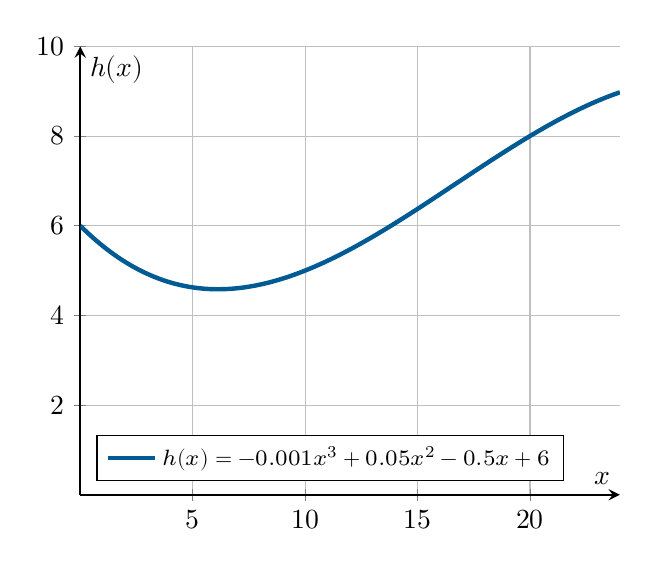
\begin{tikzpicture}
\begin{axis}[
    axis lines = center,
    xlabel = {$x$},
    ylabel = {$h(x)$},
    xmin=0.0, xmax=24,
    ymin=0, ymax=10.0,
    grid = both,
    axis line style={thick},
    legend pos=south west,
    legend style={font=\footnotesize},
    legend cell align=left,
    legend entries={$h(x) = -0.001x^3 + 0.05x^2 - 0.5x + 6$},
]
    
\addplot[draw=itwm_blue, samples=300, ultra thick, domain=0:24]{ -0.001 * x^3 + 0.05 * x^2 - 0.5 * x + 6 };
\end{axis}
\end{tikzpicture}
\end{document}